%%%%(c)
%%%%(c)  This file is a portion of the source for the textbook
%%%%(c)
%%%%(c)    Abstract Algebra: Theory and Applications
%%%%(c)    Copyright 1997 by Thomas W. Judson
%%%%(c)
%%%%(c)  See the file COPYING.txt for copying conditions
%%%%(c)
%%%%(c)
\chap{Introduction to Cryptography}{crypt}

Cryptography is the study of sending and receiving secret messages.
\footnote{Thanks to Tom Judson for material used in this chapter.}
The aim of cryptography is to send messages across a channel so only
the intended recipient of the message can read it. In addition, when a
message is received, the recipient usually requires some assurance that
the message is authentic; that is, that it has not been sent by
someone who is trying to deceive the recipient. Modern cryptography is
heavily dependent on abstract algebra and number theory. 
 
 
The message to be sent is called the \term{
plaintext}\index{Plaintext} message. The disguised message is called
the \term{ciphertext}\index{Ciphertext}. The plaintext and the
ciphertext are both written in an \term{alphabet}, consisting of \term{
letters} or \term{characters}. Characters can include not only the
familiar alphabetic characters A, $\ldots$, Z and a, $\ldots$, z but
also digits, punctuation marks, and blanks. A \term{
cryptosystem},\index{Cryptosystem!definition of} or \term{
cipher},\index{Cipher}  has two parts: \term{encryption}, the process
of transforming a plaintext message to a ciphertext message, and \term{
decryption}, the reverse transformation of changing a ciphertext
message into a plaintext message.
 
 
There are many different families of cryptosystems, each distinguished
by a particular encryption algorithm. Cryptosystems in a specified
cryptographic family are distinguished from one another by a parameter
to the encryption function called a \term{key}\index{Key!definition
of}. A classical cryptosystem has a single key, which must be kept
secret,  known only to the sender and the receiver of the message. If
person $A$ wishes to send secret messages to two different people $B$
and $C$, and does not wish to have $B$ understand $C$'s messages or
vice versa, $A$ must use two separate keys, so one cryptosystem is
used for exchanging messages with $B$, and another is used for
exchanging messages with $C$.
 
 
Systems that use two separate keys, one for encoding and another for
decoding, are called \term{public key
cryptosystems}\index{Key!public}\index{Cryptosystem!public key}. Since
knowledge of the encoding key does not allow anyone to guess at the
decoding key, the encoding key can be made public. A public key
cryptosystem allows $A$ and $B$ to send messages to $C$ using the same
encoding key.  Anyone is capable of encoding a message to be sent to
$C$, but only $C$ knows how to decode such a message.
 
 
 
\section{Private key cryptography}
 
 
In \term{single}\index{Key!single}\index{Cryptosystem!single key} or
\term{private key
cryptosystems}\index{Key!private}\index{Cryptosystem!private key}
the same key is used for both encrypting and decrypting messages. To
encrypt a  plaintext message, we apply to the message some function
which is kept secret, say $f$. This function will yield an encrypted
message.  Given the encrypted form of the message, we can recover the
original message by applying the inverse transformation $f^{-1}$. The
transformation $f$ must be relatively easy to compute, as must
$f^{-1}$; however, $f$ must be extremely difficult to guess at if only
examples of coded messages are available.
 
\subsection{Shift codes} 
 
\begin{example}{ex1}
One of the first and most famous private key cryptosystems was the
shift code used by Julius Caesar\index{Caesar, Julius}.  We first represent the alphabet numerically by
letting $\mbox{A}  = 0, \mbox{B}  = 1, \ldots, \mbox{Y} = 25, \mbox{Z} = 25$. This means for example that the word BAY would be represented numerically as:
$$ 1,0,25.$$
An example of a shift encoding function is
$$
f(p) =\bmod( p + 3,  26).
$$
which can also be written as
$$
f(p) =p \oplus 3,
$$
with the understanding that $\oplus$ refers to addition in $\mathbb{Z}_{26}$. This encoding function takes 
$$0 \rightarrow 3, 1 \rightarrow 4, \ldots, 25 \rightarrow 1,26 \rightarrow 2,$$
so that our numerical representation of BAY is changed to:  $ 4,3,1$, which is the numerical representation of EDB.

The decoding
function is the inverse of $f(p)$, which we can find by solving the equation $c = p \oplus 3$ for p.
The result is $p = c \ominus 3$, so that
$$
f^{-1}(c) = c \ominus 3 \qquad \textrm{ or }\qquad f^{-1}(c) = c \oplus 23.
$$

Suppose we receive the encoded message DOJHEUD. To decode this
message, we first represent it numerically:  
$$
3, 14, 9, 7, 4, 20, 3.
$$
Next we apply the inverse transformation to get
$$
0, 11, 6, 4, 1, 17, 0,
$$
which is the numerical representation of ALGEBRA. Notice here that there is nothing special about either of
the numbers 3 or 26. We could have used a larger alphabet or a
different shift.
\mbox{\hspace{1in}}
\end{example}

\begin{exercise}{}
\begin{enumerate}[(a)]
\item
Encode IXLOVEXMATH using the cryptosystem in Example~\ref{example:crypt:ex1}.
\item
Encode the same message using the encoding function $f(p) =p \oplus 10$.
\end{enumerate}
\end{exercise} 
 \medskip

\begin{exercise}{}
\begin{enumerate}[(a)]
\item
Decode ZLOOA WKLVA EHARQ WKHA ILQDO, which was encoded using the
cryptosystem in Example~\ref{example:crypt:ex1}.
\item
Decode: OFOBIDRSXQIYENYPVYGCPBYWDROROKBD, which was encoded using a shift code with a shift of 10.
\end{enumerate}
\end{exercise} 

\begin{exercise}{}  
\begin{enumerate}[(a)]
\item
The following is a ciphertext that was encoded using a shift code with a shift of 18.

FWHKYVOGVFGCVQWFIHOKYVQGVFGCVHSPOKYVQGVFGCV

\noindent
Find the plaintext.
\item
A plaintext is encoded using a shift code with a shift of 14. The resulting ciphertext is shift-encoded again, using a shift of 14. The result is:

VJGOQTGAQWMPQYVJGNGUUUWTGAQWCTGXQNVCKTG

\noindent
Find the plaintext.
\end{enumerate}
\end{exercise}

\term{Cryptanalysis}\index{Cryptanalysis} is concerned with
deciphering a received or intercepted message. Methods from
probability and statistics are great aids in deciphering an
intercepted message; for example, the frequency analysis of the
characters appearing in the intercepted message often makes its
decryption possible.  
 
\begin{example}{2}
Suppose we receive a message that we know was encrypted by using a
shift transformation on single letters of the 26-letter alphabet. To
find out exactly what the shift transformation was, we must compute
$b$ in the equation $f(p) = p + b \bmod 26$. We can do this using
\term{frequency analysis}\index{Frequency analysis}.  
The letter $\mbox{E} = 04$ is the most commonly
occurring letter in the English language. Suppose that $\mbox{S} = 18$
is the most commonly occurring letter in the ciphertext.  Then we have
good reason to suspect that  $18 = 4 \oplus b $, or $b= 14$.
Therefore, the most likely encoding function is
$$
f(p) = p \oplus 14.
$$
The corresponding decoding function is
$$
f^{-1}(c) = c \oplus 12.
$$
It is now easy to determine whether or not our guess is correct.
\end{example}
 
\begin{exercise}{}  
The following ciphertext was encoded using a shift code. Both the letters E and I are encoded as vowels. 

IWPDAIWPEYOEOPDAMQAAJKBPDAOYEAJYAOYWNHBCWQOO

\noindent
Find the plaintext.
\end{exercise}

\begin{exercise}{}  
In the following shift-coded ciphertext,  one of the double-letter patterns represents `ss'. 

SGD DRRDMBD NE LZSGDLZSHBR HR HM HSR EQDDCNL. FDNQF BZMSNQ

\noindent
Find the plaintext.
\end{exercise}

\begin{exercise}{}  
\begin{enumerate}[(a)]
\item
For the English alphabet, how many different shift codes are there?
\item
Thai script has 44 letters. How many different shift codes are there for the Thai language?
\end{enumerate}
\end{exercise}


\subsection{Affine codes}
 
Let us investigate a slightly more sophisticated cryptosystem. Suppose
that the encoding function is given by  
$$
f(p) = \bmod(ap + b,  26),
$$
which can also be written as
$$
f(p) = (a \odot p) \oplus b.
$$
We first need to find out when a decoding function $f^{-1}$ exists.
Such a decoding function exists when we can solve the equation
$$
c \equiv ap + b \pmod{26}\qquad \textrm{or}\qquad a \odot p = c \ominus  b
$$
for $p$ in $\mathbb{Z}_{26}$. By Proposition~\ref{proposition:modular:mod_eq_solution} in Chapter~\ref{modular}, this is possible exactly when $a$ has an
inverse in $\mathbb{Z}_{26}$, which means that $\gcd( a, 26) =1$. 
Such a cryptosystem is called an \term{affine
cryptosystem}\index{Cryptosystem!affine}. 
 
\begin{exercise}{}
\begin{enumerate}[(a)]
\item
Which of the numbers 0, 1, 2, $\dots$, 10 have inverses mod 26?
\item
For the numbers in (a) which have inverses mod 26, compute the inverses.
\end{enumerate}
\end{exercise}


\begin{exercise}{}
Find the decoding function for the following  affine encoding functions (used on the English alphabet).
\begin{enumerate}[(a)]
\item
$f(p)=3 \odot p + 14$
\item
$f(p)=5 \odot p + 15$
\item
$f(p)=7 \odot p + 23$
\end{enumerate}
\end{exercise}

\begin{exercise}{}
 Show that the  general formula for the decoding function for $f(p) = a \odot p \oplus b$ is
$$
f^{-1}(c) = (a^{-1} \odot c)  \ominus (a^{-1}\odot b).
$$
 (That is, show that $f \compose f^{-1}(c)=c$, and $ f^{-1}\compose  f(p) =  p$.)
\end{exercise}

\begin{example}{}
Let's consider the affine cryptosystem encoding function $f(p) = (a \odot p) \oplus  b$ (the $\odot$ and $\oplus$ are multiplication and addition mod 26).  For
this cryptosystem to work we must choose an $a \in {\Bbb Z}_{26}$
that is invertible. This is only possible if $\gcd(a, 26) = 1$.
Recognizing this fact, we will let $a = 5$ since $\gcd(5, 26) = 1$. The reader may check that $a^{-1} = 21$. Therefore, we can take our
encryption function to be $f(p) = (5 \odot p) \oplus 3$. Thus, ALGEBRA is
encoded as $3, 6, 7, 23, 8, 10, 3$, or DGHXIKD. The decryption
function will be   
$$
f^{-1}(p) = (21 \odot  p) \ominus (21\odot 3)  =(21 \odot  p) \oplus 15.
$$
\end{example}

\begin{exercise}{}
For each of the following functions, (i) determine whether the function is a valid encoding function; (ii) if the function is valid, find the decoding function. (Assume the function is working on an alphabet with 26 letters.)
\begin{enumerate}[(a)]
\item
$f(p) = (4 \odot p) \oplus 7$
\item
$f(p) = (5 \odot p) \oplus 13$
\item
$f(p) = (11 \odot p) \oplus 14$
\item
$f(p) = (13 \odot p) \oplus 22$
\end{enumerate}
\end{exercise}


\begin{exercise}{english}
\begin{enumerate}[(a)]
\item
The general form for an affine cryptosystem encoding function is $f(p) = (a \odot p) \oplus  b$. How many different possible values of $a$ are there, for an affine cryptosystem that works on the English alphabet of 26 letters?
\item
For the same situation as (a), how many different possible values are there for $b$?
\item
What is the total number of affine cryptosystems that work on an alphabet of 26 letters?
\end{enumerate}
\end{exercise}

\begin{exercise}{}
The Spanish alphabet has 29 letters. Give answers to parts (a), (b), and (c) of Exercise~\ref{exercise:crypt:english}, but with the Spanish alphabet instead of the English alphabet.
\end{exercise}

\begin{exercise}{}
The Hebrew alphabet has  22 letters. Give answers to parts (a), (b), and (c) of Exercise~\ref{exercise:crypt:english}, but with the Hebrew alphabet instead of the English alphabet.
\end{exercise}

\begin{exercise}{}
Suppose that the encoding function for an affine cryptosystem is $f(p) = (a \odot p) \oplus  b$, and the decoding function is 
$f^{-1}(c) = (a' \odot c) \oplus  b'$. Suppose that a different cryptosystem uses the encoding function $g(p) = (a' \odot p) \oplus  b'$. What is the decoding function for this second cryptosystem?
\end{exercise}

\begin{exercise}{}
\begin{enumerate}[(a)]
\item
The following message was encoded using an affine cryptosystem that encodes A as M and B as B. 
\medskip

CKMYCZMLCOZCWKOHUCKDOHLMZLLNMZGZOEVUFYU\\

\noindent
Find the plaintext.
\item
The following message was encoded using an affine cryptosystem that encodes A as G and C as C.
\medskip

MQTNOELNWNETEHCEWHISCFKYHHFYKGCCEIPXQWFISCF

\noindent
Find the plaintext.
\item
The following message was encoded using an affine cryptosystem that encodes R as S and S as D.
\medskip

OMFMFNSOMNDSFNDLADOMNOSFNDLAJNAALOZAUFSDONAU

\noindent
Find the plaintext.

\item
The following message was encoded using an affine cryptosystem that encodes M as N and O as D.
\medskip

NVEMBNVEHLJHJEMBNZJHLDWOBVJDI

\noindent
Find the plaintext.

\end{enumerate}
\end{exercise}

\subsection{Monoalphabetic codes}

In both shift codes and affine codes, one character in the encoded message represents exactly one character in the original message. Cryptosystems that employ such a one-to-one substitution are called \term{monoalphabetic cryptosystems}\index{Cryptosystem!monoalphabetic}.
The ``cryptoquips''\index{Cryptoquip}  that appear regularly in many newspapers make use of this type of cryptosystem (see Figure~\ref{fig:cryptoquip}).

\begin{figure}[h]
\center{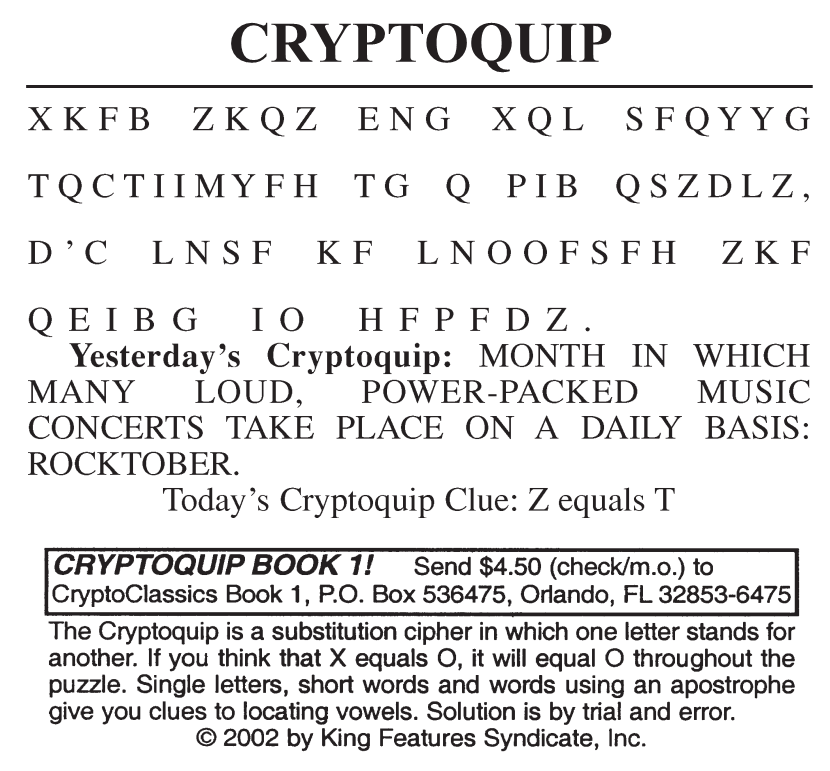
\includegraphics[width=3in]{images/cryptoquip.png}}
\caption{Example of cryptoquip (source: ``Cecil Whig'', \url{www.cecildaily.com/diversions/cryptoquip/ }).}
\label{fig:cryptoquip}
\end{figure}

\begin{exercise}{}
What is the total number of monoalphabetic cryptosystems?
\end{exercise}
Although there are many different possible monoalphabetic cryptosystems, they are relatively easy to break using frequency analysis. (You may even find web sites that can automatically decode cryptoquips.)


\subsection{Polyalphabetic codes}

A cryptosystem would be more secure if a ciphertext letter could
represent more than one plaintext letter.  To give an example of this
type of cryptosystem, called a \term{polyalphabetic
cryptosystem},\index{Cryptosystem!polyalphabetic} we will generalize
affine codes by using matrices. The idea works roughly the same as
before; however, instead of encrypting one letter at a time we will
encrypt pairs of letters.  We can store a pair of letters $p_1$ and
$p_2$ in a vector  
$$
{\bold p} = 
\left(
\begin{array}{c}
p_1 \\ p_2
\end{array}
\right).
$$
Let $A$ be a $2 \times 2$ invertible matrix
with entries in ${\Bbb Z}_{26}$. We can define an encoding function by
$$
f({\bold p}) = (A \odot {\bold p}) \oplus {\bold b} ,
$$
where ${\bold b}$ is a fixed column vector and matrix operations are
performed in ${\Bbb Z}_{26}$. The formula for  the decoding function (which is the inverse of the encoding function) is very similar to the decoding function formula that we found for affine encoding:
$$
f^{-1}({\bold p}) = (A^{-1} \odot {\bold p}) \ominus (A^{-1} \odot {\bold b}),
$$
where $A^{-1}$ is the \emph{matrix inverse} of $A$: that is, $A^{-1}A = A A^{-1} = I$, where $I$ is the $2 \times 2$ identity matrix.  *Note* that in these formulas, we are using \emph{modular} matrix multiplication instead of \emph{regular} matrix multiplication: that is, the  regular $\cdot$ and $+$ operations are replaced by  $\odot$ and $\oplus$:

\begin{exercise}{}
Perform the following operations using modular matrix multiplication (mod 26):
\begin{multicols}{2}
\begin{enumerate}[(a)]
\item
$\left(
\begin{array}{cc}
5 & 6 \\
7 & 8
\end{array}
\right)
\left(
\begin{array}{c}
4 \\
4
\end{array}
\right)$
\item
$\left(
\begin{array}{cc}
1 & 13 \\
16 & 2
\end{array}
\right)
\left(
\begin{array}{c}
3 \\
1
\end{array}
\right)$
\item
$\left(
\begin{array}{cc}
12 & 4 \\
13 & 5
\end{array}
\right)
\left(
\begin{array}{cc}
2 &1 \\
20 & 20 
\end{array}
\right)$
\item
$\left(
\begin{array}{cc}
13 & 2 \\
2 & 13
\end{array}
\right)
\left(
\begin{array}{cc}
2 &13 \\
13 & 2 
\end{array}
\right)$
\end{enumerate}
\end{multicols}
\end{exercise} 
 
\begin{example}{4}
Suppose that we wish to encode the word HELP. The corresponding
digit string is $7, 4, 11, 15$. If
$$
A =
\left(
\begin{array}{cc}
3 & 5 \\
1 & 2
\end{array}
\right),
$$
then
$$
A^{-1} 
=
\left(
\begin{array}{cc}
2 & 21 \\
25 & 3
\end{array}
\right).
$$
(You may check that $\bmod(AA^{-1},26) = \bmod(A^{-1}A,26) = I$.)
If ${\bold b} = \left( \begin{array}{c} 2 \\ 2 \end{array} \right)$, then our message is encrypted as
RRGR, where HE encrypts as RR and LP encrypts as GR.
\end{example}
In order to make use of polyalphabetic cryptosystems, we need to be able to find the inverse of a $2 \times 2$ matrix
with entries in ${\Bbb Z}_{26}$. As we *noted* above, this inverse is under matrix multiplication mod 26, rather than regular matrix multiplication.
Still, we can try to make use of the matrix inverse formula from regular matrix multiplication:
$$
\left( \begin{array}{cc} a & b \\ c & d \end{array} \right)^{-1}
= \frac{1}{ad-bc} \left( \begin{array}{cc} d & -b \\ -c & a \end{array} \right)  =  \left( \begin{array}{cc} kd & -kb \\ -kc & ka \end{array} \right),
$$
where 
$$ k = \frac{1}{ad - bc}.$$
This suggests that the following formula may be valid mod 26:
$$
\left( \begin{array}{cc} a & b \\ c & d \end{array} \right)^{-1}
=
\left( \begin{array}{cc} k \odot d & -k \odot b \\ -k \odot c & k \odot a \end{array} \right),
$$
where 
$$ k = ((a \odot d) \ominus (b \odot c))^{-1},$$
and $(\cdots)^{-1}$ means inverse under multiplication in ${\Bbb Z}_{26}$. 
We will see in the following exercise that  this works as long as $(a \odot d) \, \ominus \, (b \odot c)$ has a multiplicative inverse in ${\Bbb Z}_{26}$.

\begin{exercise}{}
Suppose that $(a \odot d) \, \ominus \, (b \odot c)$ has an inverse in ${\Bbb Z}_{26}$: that is to say, suppose there is a $k \in  {\Bbb Z}_{26}$ such that $k \odot ((a \odot d) \, \ominus \, (b \odot c)) = 1$.  Show that the matrices:
$$
A = \left( \begin{array}{cc} a & b \\ c & d \end{array} \right)~~~\text{and}~~~
B=
\left( \begin{array}{cc}  k \odot d & - k \odot b \\ - k \odot c &  k \odot a \end{array} \right)$$
are inverses of each other  in ${\Bbb Z}_{26}$.  That is, show that $AB = BA = I$ under matrix multiplication mod 26.

\end{exercise} 
The previous exercise leaves open the question of whether $\left( \begin{array}{cc} a & b \\ c & d \end{array} \right)$ has an inverse when $(a \odot d)  \ominus (b \odot c)$ has no inverse in ${\Bbb Z}_{26}$. Once again, we can reach back to our previous matrix knowledge to resolve this issue. Recall that the quantity $ad - bc$ is called the \term{determinant}\index{Matrix!determinant} of the matrix  $\left( \begin{array}{cc} a & b \\ c & d \end{array} \right)$.  There is also a famous formula for the determinant of the product of matrices:
$$\text{det}(A) \text{det}(B) = \text{det}(AB).$$
This same formula carries over to matrix multiplication mod 26, because (as we've seen) in any equation using only the operations of multiplication, addition, and subtraction, we can replace these operations with their modular versions and still have a true equation. We can use this to show that $(a \odot d)  \ominus (b \odot c)$ \emph{must} have an inverse in ${\Bbb Z}_{26}$ in order for $\left( \begin{array}{cc} a & b \\ c & d \end{array} \right)$ to have an inverse:

\begin{exercise}{mat1}
Suppose that $A = \left( \begin{array}{cc} a & b \\ c & d \end{array} \right)$ is a matrix with entries in ${\Bbb Z}_{26}$, such that  $(a \odot d)  \ominus (b \odot c)$ has no inverse in ${\Bbb Z}_{26}$. Show that $A$ has no inverse in  ${\Bbb Z}_{26}$.
\hyperref[sec:crypt:hints]{(*Hint*)}
\end{exercise}


\begin{exercise}{minv}
Find matrix inverses in ${\Bbb Z}_{26}$ for the following matrices. If no inverse exists, then prove there is no inverse.
\begin{multicols}{2}
\begin{enumerate}[(a)]
\item
$\left( \begin{array}{cc} 9 & 2 \\ 20 & 31 \end{array} \right)$
\item
$\left( \begin{array}{cc} 2 & 3 \\ 23 & 2 \end{array} \right)$
\item
$\left( \begin{array}{cc} 4 & 11 \\ 3 & 2 \end{array} \right)$
\item
$\left( \begin{array}{cc} 2 & 2 \\ 3 & 4 \end{array} \right)$
\end{enumerate}
\end{multicols}
\end{exercise}
 \begin{exercise}{}
For the same matrices as in Exercise~\ref{exercise:crypt:minv}, find the matrix inverses in ${\Bbb Z}_{29}$.
\end{exercise}

\begin{exercise}{}
Given that
$$
A =
\left(
\begin{array}{cc}
3 & 4 \\
2 & 3
\end{array}
\right),~~ \text{and~} {\bold b} = \left( \begin{array}{c} 2 \\ 5 \end{array}\right).$$
\begin{enumerate}[(a)]
\item
Use the encryption function $f({\bold p}) = A {\bold p} + {\bold b}$
to encode the message CRYPTOLOGY.  
\item
What is the decoding function?  
\end{enumerate}
 \end{exercise}
 
Frequency analysis can still be performed on a polyalphabetic
cryptosystem, because we have a good understanding of how pairs of
letters appear in the English language. The pair {\em th} appears
quite often; the pair {\em qz} never appears.  To avoid decryption by
a third party, we must use a larger matrix than the one we used in
Example~\ref{example:crypt:4}. 
  
\subsection{Spreadsheet exercises}
Spreadsheets can be used to automate many of the calculations that we have looked at in the previous sections.

\begin{exercise}{EngShift}
In this exercise, you will use a spreadsheet to create an automated shift encoder for English. Please refer to Figure~\ref{fig:AutoShiftEnc} for guidance:
\begin{figure}[h]
\center{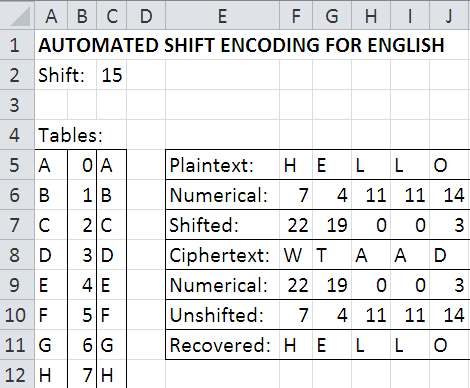
\includegraphics[width=3.0in]{images/AutoShiftEnc.png}}
\caption{Automatic shift encoder for English.}
\label{fig:AutoShiftEnc}
\end{figure}
\begin{enumerate}[(i)]
\item
Put the Shift value in cell C2.
\item
Put the alphabet (starting with A), numerical values for the letters (starting with 0), and the alphabet again in columns A, B, C starting on line 5.
\item
Type your plaintext in row 5, starting in column F.
\item
Row 6 beginning in column F contains the numerical values for the plaintext. The formula in cell F6 is: ``=VLOOKUP(F5, \$A\$5:\$B\$30,2)''. The significance of this formula is as follows:
\begin{itemize}
\item
The function VLOOKUP means that the program will look up a given value in a given table;
\item
The F5 is the first argument of VLOOKUP, which means that the value being looked up is in cell F5;
\item
The \$A\$5:\$B\$30 is the second argument of VLOOKUP, which means that it represents the cells containing the table that the value will be looked up in.  The dollar signs are used to guarantee that the table will remain fixed when the formula is copied and pasted into another cell;
The 2 which is the third lookup of VLOOKUP indicates that the value in the second column in the same row as the looked-up value is placed in the cell where the formula is located.
\end{itemize}
\item
Row 7 beginning in column F gives the encoded numerical values. The formula in cell F7 is ``=MOD(F6+\$C\$2,26)''.  The dollar signs on C2 guarantee that when the formula is copied, the shift still refers to the value in C2.
\item
Row 8 beginning in column F gives the ciphertext.  The formula in cell F8 is: ``=VLOOKUP(F7,\$B\$5:\$C\$30,2)''. 
\item
Rows 9,10, and 11 are similar to rows 6,7,8 respectively. Try to do this yourself. 
\end{enumerate}
Once you have completed the formulas, select cells F6 through J11, and use the spreadsheet's ``Fill Right'' capability to carry the formulas to the other columns.  (If your plaintext is longer, you can select more columns and fill right.
\end{exercise}

\begin{exercise}{}
The Spanish alphabet has 3 more letters than English:  `Ch' (comes after C in the alphabet), `Ll'  (comes after L in the alphabet), and `Nn' (comes after N).  Modify the sheet you created in Exercise \ref{exercise:crypt:EngShift} to make a Spanish language shift encoder.  Use your sheet to decode the following message:

MS KIUPVA	UID NIKPS VA MD DPMUBChM MS UMQACh

(Note that `Ch' counts as a single letter.)
\end{exercise}

\begin{exercise}{}
Create a spreadsheet that can perform any affine encoding on English plaintext.  You may model your spreadsheet on the sheet in Figure~\ref{fig:affine}.  Use your spreadsheet to decode the following message:


EMBNDOBFDZXIDPEMBSBJJJZOBFDZVOBUDSEVHOB

which was encoded using an affine encoding function with $b=21$.
\begin{figure}[h]
\center{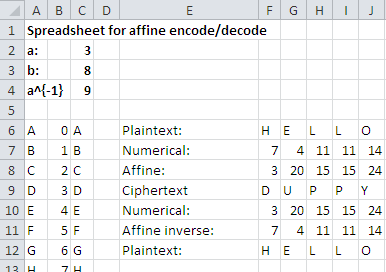
\includegraphics[width=3.5in]{images/Affine.png}}
\caption{Automatic affine encoder for English.}
\label{fig:affine}
\end{figure}
\end{exercise}

\begin{exercise}{}
In order to decode an affine cryptosystem on English letters with encoding function $f(p) = (a\odot p) \oplus b$, it is necessary to find the inverse of $a$ under multiplication mod 26. We have ways of finding inverses of individual numbers.  But we can also use spreadsheet software  to find all inverses in one fell swoop as described below.

Open a sheet in  your favorite spreadsheet software (Excel, LibreOffice, or OpenOffice). Put the numbers 0 through 25 in column A, starting at row 3, and also in row 2 starting in column B. To fill up the table, put the formula ``=MOD(\$A3*B\$2,26)'' in cell B3, as shown in Figure~\ref{fig:mod26mult}. This formula causes the software to take the product of the contents of cells A3 and B2, and put the result mod 26 into cell B3.  The dollar signs are important: these indicate ``fixed reference''.  For example, the `\$A3' means that when this formula is copied to other cells, the reference to column A remains unchanged while the column may change. On the other hand, the `B\$2' means that when the formula is copied to other cells, the reference to column 2 remains unchanged.

At this point, select the range of cells from B3 to AA28 (this will be a  square region of $26 \times 26$ cells. Use your spreadsheet's ``Fill down'' and ``Fill right'' feature to fill all the cells in this region. The location of all of the `1''s in this table shows all of the inverses.  For example, there is a '1' in the row labeled 9 and column labeled 3.  This means that 9 and 3 are inverses of each other mod 26.

Use this spreadsheet table to create a 2-column table: in the first column, put the numbers 0 through 26, and in the second column, put the inverses (if the number has no inverse, just put a `$-$').
\begin{figure}[h]
\center{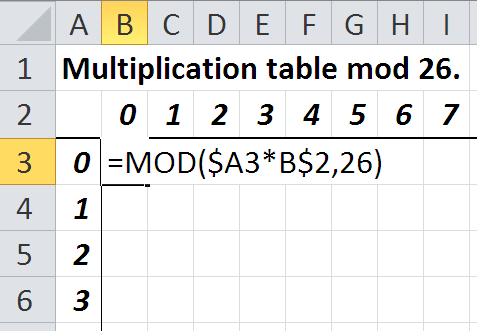
\includegraphics[width=2.25in]{images/MultMod26.png}}
\caption{Mod 26 multiplication table.}
\label{fig:mod26mult}
\end{figure}
\end{exercise}

\begin{exercise}{}
Following the previous exercise, find all inverses of the numbers mod 29 (this can be used in affine encoding of Spanish, which has 29 letters).
\end{exercise}

\begin{exercise}{}
Make a spreadsheet that can do polyalphabetic coding.  you may base your sheet's design on Figure~\ref{fig:polycrypto}. The figure shows the encoding of the word CRYPTOLOGY using 
$A = \left(
\begin{array}{cc}
3 & 5 \\
1 & 2
\end{array}
\right)$, and ${\bold b} = \left( \begin{array}{c} 2 \\ 2 \end{array}\right).$ 

Use your spreadsheet to decode the following words that were encoded using $f({\bold p}) = A {\bold p} + {\bold b}$ with the given $A$ and ${\bold b}$.
\begin{enumerate}[(a)]
\item
VVDGOFOKLY, $A= \left(
\begin{array}{cc}
13 & 5 \\
9 & 2
\end{array}
\right)$, and ${\bold b} = \left( \begin{array}{c} 7 \\ 13 \end{array}\right).$ 
\item
VWFGTWQKTA, $A= \left(
\begin{array}{cc}
17 & 13 \\
6 & 3
\end{array}
\right)$, and ${\bold b} = \left( \begin{array}{c} 14 \\ 18 \end{array}\right).$ 
\item
EXUFQPRRGA, $A= \left(
\begin{array}{cc}
3 & 4 \\
5 & 7
\end{array}
\right)$, and ${\bold b} = \left( \begin{array}{c} 4 \\ 8 \end{array}\right).$ 
\end{enumerate}
\begin{figure}[h]
\center{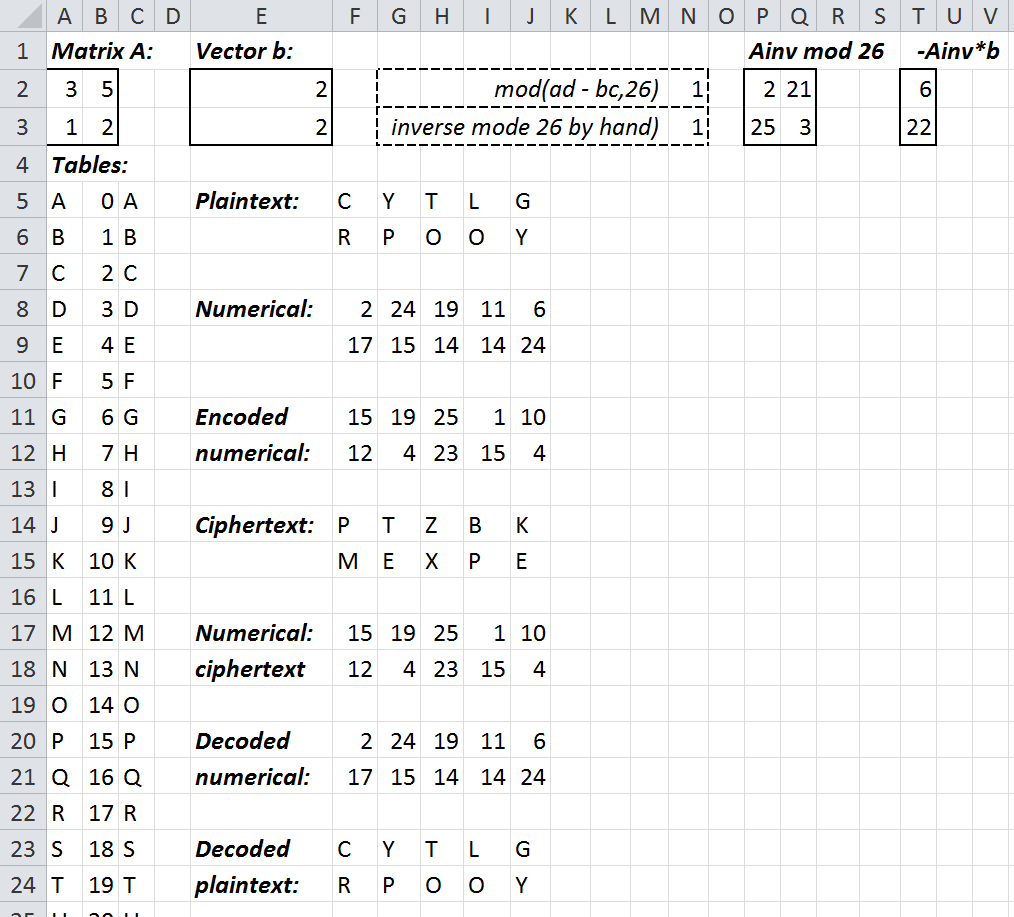
\includegraphics[width=5in]{images/polycrypto2.png}}
\caption{(Semi-)automatic polyalphabetic encoder/decoder for English. Note that cell N3 is entered by hand, based on the value in N2.}
\label{fig:polycrypto}
\end{figure}
\end{exercise}


\section{Public key cryptography}
  
If traditional cryptosystems are used, anyone who knows enough to
encode a message will also know enough to decode an intercepted
message. In 1976, W.~Diffie\index{Diffie, W.} and
M.~Hellman\index{Hellman, M.} proposed public key cryptography, which
is based on the observation that the encryption and decryption
procedures need not have the same key. This removes the requirement
that the encoding key be kept secret. The encoding function $f$ must
be relatively easy to compute, but $f^{-1}$ must be extremely
difficult to compute without some additional information, so that
someone who knows only the encrypting key cannot find the decrypting
key without prohibitive computation. It is interesting to note that to
date, no system has been proposed that has been proven to be
``one-way;'' that is, for any existing public key cryptosystem, it has
never been shown to be computationally prohibitive to decode messages
with only knowledge of the encoding key. 
 
 
 
\subsection{The RSA cryptosystem}\label{sec:RSA}
 
The RSA cryptosystem introduced by R.~Rivest\index{Rivest, R.},
A.~Shamir\index{Shamir, A.}, and L.~Adleman\index{Adleman, L.} in
1978, is based on the difficulty of factoring large numbers. Though it
is not a difficult task to find two large random primes and multiply
them together, factoring a 150-digit number that is the product of two
large primes would take 100 million computers operating at 10 billion
instructions per second about 50,000 years under the fastest
algorithms currently known.
 
Let us look at how RSA works in a practical context.  
Suppose that Jennifer is running an online boutique, and wants to receive
 credit card information from customers over the internet. Unfortunately it's all too easy to snoop the internet, 
and it certainly wouldn't be good for Jennifer's customers if their credit card numbers were stolen. 
So she needs a suitable code for the credit card information in order to protect her customer's privacy.
The code may be constructed as follows:
\begin{enumerate}[(a)]
\item 
Choose  two random 150-digit prime
numbers $p$ and $q$. (This is easier said than done!  We will consider some possible ways of doing this in Section~\ref{primality}.)
\item
Compute the product $n= pq$ as well as $ m = (p - 1)(q-1)$. 
(It can be shown that $m$ is actually the number of positive integers in $\mathbb{Z}_n$ that are relatively prime to $n$.)    
\item
Find a large random integer $E$ that is relatively prime to $m$. This is done by making a guess for $E$, then using the Euclidean algorithm to check whether $\gcd(E, m) = 1$. If not, then keep guessing until you find an $E$ that works. In general relatively prime numbers are not uncommon, and the Euclidean algorithm is pretty quick (especially for a computer), so $E$ is not too difficult to find.  
\item
Using the Euclidean algorithm, find $D$ such that \mbox{$DE \equiv 1 \pmod{m}$}. 
\end{enumerate}
 Now, let's say that Jennifer has a  customer whose credit card number is $x$.  Before requesting the credit card information, Jennifer's computer  sends the numbers  $E$ and $n$ to the customer's computer, which then calculates $y = x^E \mod n$ and sends $y$ to
Jennifer's computer, Jennifer recovers $x$ by computing  $y^D \bmod
n$, which (as we shall show in a minute) turns out to be $x$, as long as $x$ is less than $n$. 

Notice some amazing things here. First, $E$ and $n$ are sent out \emph{openly} over the internet. Jennifer doesn't care if  snoopers find out this information. In fact, she sends the \emph{same} $E$ and $n$ to each customer! But this does not compromise her customers' security, because only Jennifer knows $m$, and it takes both $E$ and $m$ to find $D$. As long as no one can figure out $m$, the credit card numbers are safe!

To summarize: once the public key $(E,n)$ and the private key $D$ have been constructed, the process of encoding and decoding is simple:
\begin{itemize}
\item
To encode a numerical plaintext $x$:  compute $\mod (x^E,n)$ .
\item
To decode a numerical ciphertext $y$: compute $\mod(y^D,n)$.
\end{itemize}
 
\vspace{2 ex}
 
\begin{example}{}
Before exploring the theory behind the RSA cryptosystem or attempting
to use large integers, we will use some small integers just to see
that the system does indeed work. Suppose that we wish to send some
message, which when digitized is 395. Let $p = 23$ and $q = 29$.  Then 
$$ n = pq = 667 \qquad \textrm{and} \qquad
m = (p - 1)(q - 1) = 616.
$$
We can let $E = 487$, since $\gcd(616, 487) = 1$. The encoded message
is computed to be  
$$
\bmod(395^{487},  667) = 570.
$$
(This may seem like a very long computation, but there are fast ways of doing this: see Exercise \ref{exercise:crypt:power} below.)
Using the Euclidean
algorithm, we determine that $191 E = 1 + 151 m$; therefore, the
decrypting key is $(n, D) = ( 667, 191)$. We can recover the original 
message by calculating  
$$
 \bmod(570^{191}, 667) = 395.
$$
\end{example}
 
 
\vspace{ 2 ex}
 
 
This really seems like magic. How in the world does it work? 
First of all, we know that $DE
\equiv 1 \bmod{ m}$; so there exists a $k$ such that 
$$
DE = km + 1.
$$
This means that
$$
y^D = (x^E)^D = x^{DE} = x^{km+1} = (x^m)^k x.
$$
At this point we need \emph{Euler's theorem} from Chapter~\ref{cosets}, which states the following. Suppose $m$ is the number of positive integers less than $n$ that are relatively prime to $n$. Then it is true that:
$$
x^m \equiv 1 \pmod n.
$$
for \emph{any} $x$ that is relatively prime to $n$. 

We can use this to simplify our previous expression for $y^D$:
$$
y^D =  (x^m)^k x \equiv (1)^k x  \equiv x \bmod n,
$$
 and presto! We have our result.
 
We can now ask how one would go about breaking the RSA cryptosystem.
To find $D$ given $n$ and $E$, we simply need to factor $n$ and solve
for $D$ by using the Euclidean algorithm. If we had known that $667 =
23 \cdot 29$ in Example~5, we could have recovered $D$.    
 
 
 
\begin{exercise}{primes}
Show that if $p$ and $q$ are primes, then the number of positive integers less than $pq$ which are relatively prime to $pq$ is $(p-1)(q-1)$.
\hyperref[sec:crypt:hints]{(*Hint*)}
\end{exercise}
 
\subsection{Message verification}
 
 
There is a problem of message verification in public key
cryptosystems. Since the encoding key is public knowledge, anyone has
the ability to send an encoded message.  If Alice receives a message
from Bob, she would like to be able to verify that it was Bob who
actually sent the message. Suppose that Bob's encrypting key is $(n',
E')$ and his decrypting key is $(n', D')$.  Also, suppose that Alice's
encrypting key is $(n, E)$ and her decrypting key is $(n, D)$.  Since
encryption keys are public information, they can exchange coded
messages at their convenience.  Bob wishes to assure Alice that the
message he is sending is authentic. Before Bob sends the message $x$
to Alice, he decrypts  $x$ with his own key:
$$
x' =  \bmod(x ^{D'}, n').
$$
Anyone can change $x'$ back to $x$ just by encryption, but only Bob
has the ability to form $x'$. Now Bob encrypts $x'$ with Alice's
encryption key to form 
$$
y' = \bmod({x'}^E,   n),
$$
a message that only Alice can decode.  Alice decodes the message and
then encodes the result with Bob's key to read the original message, a
message that could have only been sent by Bob.
 

\subsection{RSA exercises}
 

\begin{exercise}{power}
This problem demonstrates a fast method for computing very large powers of numbers in modular arithmetic using a spreadsheet.  You will need this method in order to do the subsequent problems. We will demonstrate the method by computing $\bmod(23^{485} ,617)$.
\begin{enumerate}[(a)]
\item
Use a spreadsheet to compute the following sequence of numbers:
\[ 23, \bmod(23^2 ,617),\bmod(23^4 ,617),\ldots,\bmod(23^{256} ,617) \]
Note that each power of 23 in this series is the  \emph{square} of the previous power.  So to compute any number in this series, square the previous number and reduce mod 617.  You may use the MOD spreadsheet function.  It is easiest to put all the numbers in a single column. (This way, you can use the spreadsheet's ``Fill down'' feature.)
\item  Write 485 as a sum of powers of 2.  (This is the same thing as finding the \emph{binary expansion} of 485.)
\item Using the results of (b), identify a set of entries from the table you found in part (a), such that the product of these entries is equivalent to $23^{485}  \pmod{617}$.
\hyperref[sec:crypt:hints]{(*Hint*)}
\item 
Use your result from (c) to compute $\bmod(23^{485} ,617)$.
\end{enumerate}
\end{exercise}

\begin{exercise}{powerplus}
Building off the previous exercise, create a spreadsheet that can compute $\bmod(n^{q},b)$ for general $n,q,b$.  You may follow the pattern of the spreadsheet in Figure~\ref{fig:LargePowMod}.  Some of the formulas in the spreadsheet are:
\begin{itemize}
\item
Cell A8: ~~=B3
\item
Cell B8: ~~=MOD(A8,2)
\item
Cell A9: ~~=(A8 - B8)/2
\item
Cell D9: ~~ = D8*2
\item
Cell E9: ~~ = MOD(E8*E8, \$B\$4)
\item
Cell F8: ~~ = B8
\item
Cell G8: ~~ = E8$\widehat{~~}$F8
\item
Cell H8: ~~ = G8
\item
Cell H9: ~~ = MOD(G9*H8,\$B\$4)
\end{itemize}
You may obtain the rest of the formulas using the spreadsheet's ``fill down'' capability.

\begin{figure}[h]
\center{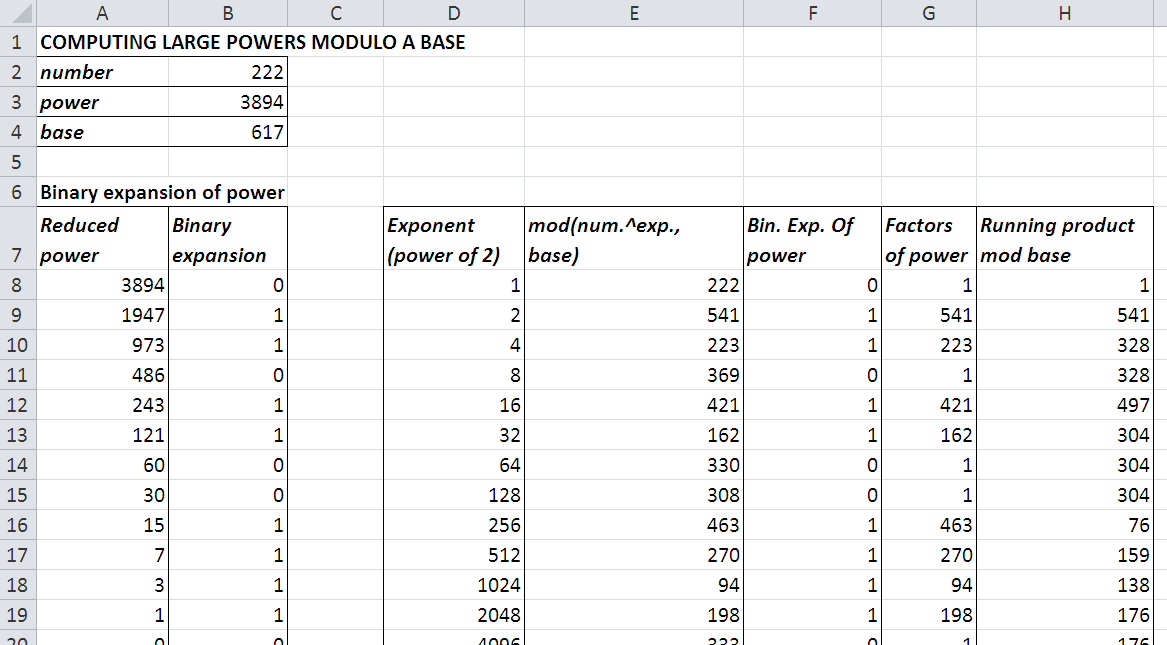
\includegraphics[width=5.5in]{images/LargePowMod.png}}
\caption{Spreadsheet for taking large powers modulo a given base.}
\label{fig:LargePowMod}
\end{figure}
\end{exercise} 


\begin{exercise}{RSA_E}
Encrypt each of the following RSA messages $x$ so that $x$ is divided
into blocks of integers of length 2;  that is, if $x = 142528$, encode 
14, 25, and 28 separately.
 
\vspace{3pt}        %two column exercise list
 \hspace{-7pt}
\begin{minipage}[t]{4.6in}
\noindent
\begin{minipage}[t]{2.25in}
\begin{itemize}
 
 \item[{\bf (a)}]
$n = 3551, E = 629, x = 31$
 
 \item[{\bf (c)}]
$n = 120979, E = 13251,\\ x = 142371$
 
\end{itemize}
\end{minipage} \hfill
\begin{minipage}[t]{2.25in}
\begin{itemize}
 
 \item[{\bf (b)}]
$n = 2257, E = 47, x = 23$
 
 \item[{\bf (d)}]
$n = 45629, E = 781,\\ x = 231561$
 
\end{itemize}
\end{minipage}
\end{minipage}
\end{exercise}
 
\begin{exercise}{}
Decrypt each of the following RSA messages $y$. (In this case, do not break $y$ into blocks--decode the entire number.)
 
 \begin{enumerate}[(a)]
\item
 $n = 3551, D = 1997, y = 2791$
 \item
$n = 5893, D = 81, y = 34$
 \item
$n = 120979, D = 27331, y = 112135$
 \item
$n = 79403, D = 671, y = 129381$
 \end{enumerate}
 \end{exercise}
 
%\begin{exercise}{}
%For each of the following encryption keys $(n, E)$ in the RSA
%cryptosystem, compute $D$.(\emph{Hint}
% 
%\vspace{3pt}        %two column exercise list
% 
%\hspace{-7pt}
%\begin{minipage}[t]{4.6in}
%\noindent
%\begin{minipage}[t]{2.25in}
%\begin{itemize}
% 
% \item[{\bf (a)}]
%$(n, E) = (451, 231)$
% 
% \item[{\bf (c)}]
%$(n, E) = (37986733, 12371)$
% 
%\end{itemize}
%\end{minipage} \hfill
%\begin{minipage}[t]{2.25in}
%\begin{itemize}
% 
% \item[{\bf (b)}]
%$(n, E) = (3053, 1921)$
% 
% \item[{\bf (d)}]
%$(n, E) =\\ (16394854313, 34578451)$
% 
%\end{itemize}
%\end{minipage}
%\end{minipage}
% 
%\vspace{2pt}        %end two column exercise list
% \end{exercise}
 
\begin{exercise}{} 
Encrypted messages are often divided into blocks of $n$ letters. A
message such as THE WORLD WONDERS WHY might be encrypted as 
JIW OCFRJ LPOEVYQ IOC but sent as JIW OCF RJL POE VYQ
IOC.  What are the advantages of using blocks of $n$ letters? 
 \end{exercise}
 
 
\begin{exercise}{}
Construct an RSA cryptosystem as follows:
\begin{enumerate}[(a)]
\item
On the web, find two four-digit primes
\item
Use these primes to compute $n$ and $m$.
\item
Choose a value of $E$ which is less than $m$, and use you Diophantine Equation spreadsheet (Exercise~\ref{exercise:modular:DiophantineSS} in the Modular Arithmetic chapter) to find the inverse $D$ under multiplication mod $m$.  If it turns out that $E$ is not relatively prime to $m$, try again.
\item
Test your cryptosystem by encoding `123', and then decoding it. To encode, use the spreadsheet that you 
created in Exercise~\ref{exercise:crypt:powerplus} earlier in this chapter. To decode, make another copy of the same sheet.
\end{enumerate}
\end{exercise} 
 
 
\subsection{Additional exercises: identifying prime numbers}\label{primality}
 
We saw in Section~\ref{sec:RSA} that the RSA algorithm depends on finding very large primes. In practice, large primes are found using trial and error. That is, we choose a large random number and test to see whether it's prime. 
If the test fails, then try, try again.

So it all comes down to figuring out how to test whether a number is prime. In this section, we consider some possible ways of doing this.

\subsubsection*{\emph{``Brute force'' method, and sieve of Eratosthenes}}
On way to do this is sheer brute force: try dividing by 2,3,4, $\ldots$, and if nothing divides then the number is prime. There are various ways to make this process more efficient, as we will see in the following exercises.

\begin{exercise}{brute}
To test whether the number $n$ is a prime, you divide $n$ all the integers $1,2,3, \dots$ up to $a$, and see if any of them divides evenly.  How large does $a$ have to be in order to guarantee that $n$ really is a prime?
\hyperref[sec:crypt:hints]{(*Hint*)}
\end{exercise}

When testing whether $n$ is prime, by the ``brute force'' method, as long as $n$ is odd we don't need to divide by even numbers (Why?). 
This means that you only need to test about half of the numbers up to $a$--more precisely, we only need to test $\lceil a/2 \rceil$ numbers, where $\lceil x \rceil$ means ``the next integer larger than $x$''. ($\lceil x \rceil$ is called the \emph{ceiling} of $x$.\index{Ceiling!of a real number}) 

We can pull the same trick with factors that are divisible by 3.  Once we've tested 3 as a factor, we don't need to check $9, 15, 21, \ldots$ or any other number that is divisible by 3.  (Why?)  So it seems that this reduces the number of factors that we need to check by about a third, since every third integers are divisible by 3. However, we need to be careful here. We've already ruled out the numbers that are divisible by 2, so the numbers that are divisible by both 2 and 3 have already been ruled out. In other words (using $m$ to denote a positive integer, and using the the notation $| \{ \cdots \} |$ to denote the size of sets):
\begin{align*}
&| \{ m \le a \text{ and } (2 \mid m \text{ or } 3 \mid m) \}| =\\ 
&~~~| \{ m \le a  \text{ and } 2 \mid m \}| + | \{ m \le a  \text{ and } 3 \mid m \}| - | \{ m \le a  \text{ and } 6 \mid m \}|.
\end{align*}
If we are not so careful with the ``ceiling function'' (which changes the result by at most 1 anyway), this tells us:
\begin{align*}
| \{ m \le a \text{ and } 2 \mid m \text{ or } 3 \mid m \}| &\approx 
\frac{a}{2} + \frac{a}{3} -\frac{a}{6}.
\end{align*}
We can turn this around and find the number of integers which are \emph{not} divisible by 2 or 3:
\begin{align*}
| \{ m \le a \text{ and } 2 \nmid m \text{ and } 3 \nmid m \}| &\approx 
a - \frac{a}{2} - \frac{a}{3} + \frac{a}{6} \\
&\approx a\left(1 - \frac{1}{2}\right) \left(1 - \frac{1}{3}\right)\\
&\approx \frac{a}{3}.
\end{align*}
This gives the number of trial divisions required to test whether $n$ is prime. (Of course we also need to test divisibility by 2 and 3, which are 2 additional divisions.)

The same reasoning can be extended to take into account divisibility by 5, 7, 11, and so on:

\begin{exercise}{EulerTotient}
Using the same reasoning as above, show that after dividing by $2,3,5$ the number of additional divisions required to test for primality is:
$$a\left(1 - \frac{1}{2}\right) \left(1 - \frac{1}{3}\right)\left( 1 - \frac{1}{5} \right).$$
\end{exercise}

It turns out that the formula in Exercise~\ref{exercise:crypt:EulerTotient} can be generalized. The resulting function of $a$ when \emph{all} primes less than $a$ are taken into account is called the \term{Euler totient function}. \index{Euler! totient function}
The technique of eliminating numbers to check based on previous divisibility is called the \term{sieve of Eratosthenes}\index{Sieve of Eratosthenes}.


\subsubsection*{\emph{Fermat's test for primality}}
Even using various tricks to reduce the number of computations, the brute force method requires far too many calculations to be useful for RSA encoding. A different algorithm for testing primality is \term{
Fermat's factorization algorithm}\index{Fermat!factorization
algorithm}, which depends on the following fact:

\begin{exercise}{Fermat}
Let $n= ab$ be an odd composite number. Prove that $n$ can be written
as the difference of two perfect squares:
$$
n = x^2 - y^2 = (x-y)(x+y).
$$
Consequently, a positive odd integer can be factored exactly when we
can find integers $x$ and $y$ such that $n = x^2 - y^2$.
\hyperref[sec:crypt:hints]{(*Hint*)} 
\end{exercise} 
We can use this fact to factor $n$ by trying different pairs of squares in order to get $n$ as the difference of the two.  Of course, we want to do this systematically. So we want to see what values of $x$ and $y$ we actually need to check:

\begin{exercise}{smallest_value}
In the formula  $n = x^2 - y^2 = (x-y)(x+y)$,  what is the smallest possible value for $x$ that needs to be tested?
\hyperref[sec:crypt:hints]{(*Hint*)}
\end{exercise}

There are other special conditions that $x$ and $y$ must satisfy:

\begin{exercise}{FermatEfficient}
\begin{enumerate}[(a)]
\item
Assuming that $n$ is an odd number, show that if $x$ is odd then $y$ is even, and if $x$ is even then $y$ is odd.
\hyperref[sec:crypt:hints]{(*Hint*)}
\item
Show that for any odd number $m$, then $\mod(m^2,4) = 1$.
\hyperref[sec:crypt:hints]{(*Hint*)}
\item
Let $m = x + y$. Show that $m$ is odd, and that we can rewrite  $n  = (x-y)(x+y)$ as: $n = m(m-2y)$. 
\item
Show that if $\mod(n,4)=1$, then $y$ must be even.
\hyperref[sec:crypt:hints]{(*Hint*)}
\item
Show that if $\mod(n,4)=3$, then $y$ must be odd.
\hyperref[sec:crypt:hints]{(*Hint*)}
\end{enumerate}
\end{exercise}

The Fermat primality testing scheme is better for finding factors that are nearly equal. The brute force method of Exercise~\ref{exercise:crypt:brute}  is much better when one factor is much better than the other one.

\begin{exercise}{}
\begin{enumerate}[(a)]
\item
Create a spreadsheet that factors large numbers using the brute force scheme. You may use the spreadsheet in Figure~\ref{fig:bf} for inspiration. Some of the formulas in the spreadsheet are:
\begin{itemize}
\item
Cell A7: ~~=A6+2
\item
Cell B6:  ~~=\$B\$2/A6
\item
Cell C6:  ~~=IF(B6=FLOOR(B6,1),A6,0)
\item
Cell E2: ~~=MAX(C6:C99999)
\end{itemize}
You may obtain the rest of the formulas using the spreadsheet's ``fill down'' capability.
\item
Use this spreadsheet to factor $n=3551$. Then, use your result to find the decoding key $D$ for Exercise~\ref{exercise:crypt:RSA_E} part (a).
\item
Use this spreadsheet to  find the decoding key $D$ for Exercise~\ref{exercise:crypt:RSA_E} part (b).
\item
Use this spreadsheet to  find the decoding key $D$ for Exercise~\ref{exercise:crypt:RSA_E} part (c).
\item
Use this spreadsheet to  find the decoding key $D$ for Exercise~\ref{exercise:crypt:RSA_E} part (d).
\item
Given the encryption key $(n,E) = (451,231)$, find $D$.
\item
Given the encryption key $(n,E) = (3053,1921)$, find $D$.
\end{enumerate}
\end{exercise}

\begin{figure}[h]
\center{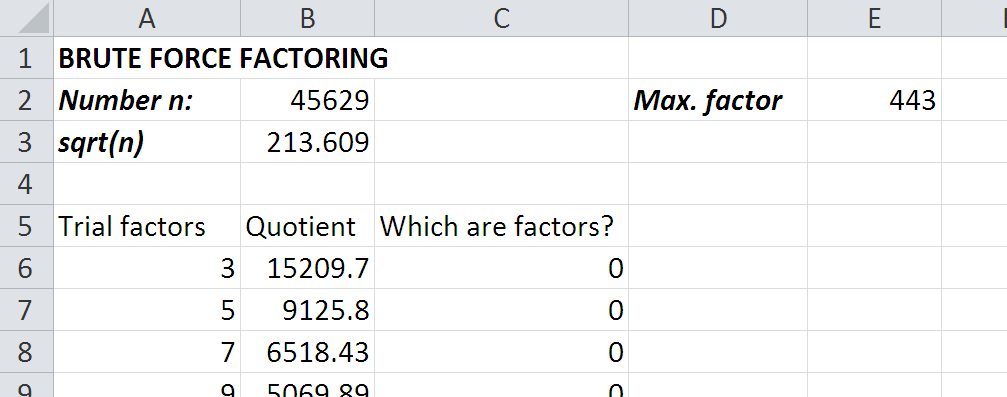
\includegraphics[width=4in]{images/bf.png}}
\caption{Spreadsheet for brute force factoring method}
\label{fig:bf}
\end{figure}


\begin{exercise}{FermatSpreadsheet}
\begin{enumerate}[(a)]
\item
Make a spreadsheet for Fermat's factoring method. You may use the spreadsheet in Figure~\ref{fig:FermaFact} for inspiration. Some of the formulas in the spreadsheet are:
\begin{itemize}
\item
Cell A7: ~~=A6+1
\item
Cell B6:  ~~=SQRT(A6*A6 - \$B\$2)
\item
Cell C6:  ~~=IF(B6=FLOOR(B6,1),A6-B6,0)
\item
Cell D6:  ~~=IF(B6=FLOOR(B6,1),A6+B6,0)
\item
Cell E2: ~~=MAX(C6:C99999)
\item
Cell F2: ~~=MAX(D6:D99999)
\end{itemize}
You may obtain the rest of the formulas using the spreadsheet's ``fill down'' capability.
\item
Use this spreadsheet to factor $n=7433551$. Then, use your result to find the decoding key $D$ for $(n,E) = (7433551,12345)$.
\item
Use this spreadsheet to factor $n=16394854313$. Then, use your result to find the decoding key $D$ for $(n,E) = (16394854313,34578451)$. 
\end{enumerate}
\end{exercise}


\begin{figure}[h]
\center{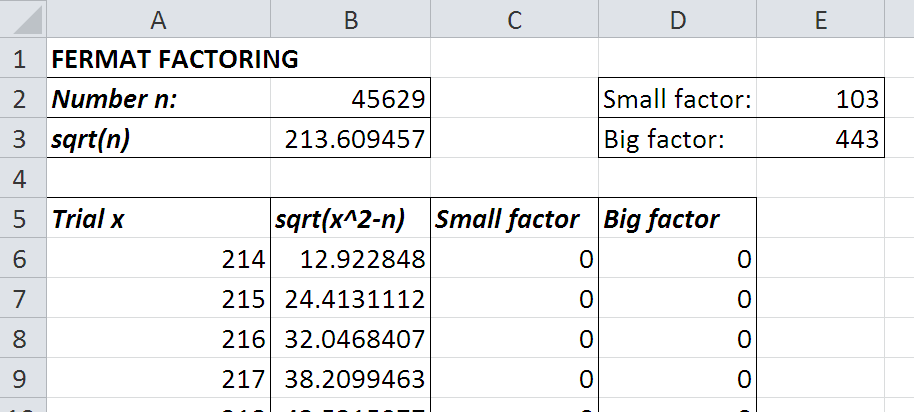
\includegraphics[width=4in]{images/FermaFact.png}}
\caption{Spreadsheet for Fermat difference-of-squares factoring method}
\label{fig:FermaFact}
\end{figure}

\begin{exercise}{}
* Using the results from Exercise~\ref{exercise:crypt:FermatEfficient} parts (d) and (e), modify the spreadsheet that you created in Exercise~\ref{exercise:crypt:FermatSpreadsheet} to make it twice as efficient.  In other words, modify the formula in cell A6 so that you can replace the formula in A7 with the formula: `=A6+2'.
\end{exercise}

\subsubsection*{\emph{Probabilistic methods using the ``little Fermat theorem''}}
In practice, neither the brute force nor the Fermat method is used to verify large prime numbers. Instead, 
\emph{probabilistic methods} are used: these methods can show that it's very, very likely that $n$ is a prime, but they don't prove for certain. The principal test of this type is the  \term{Miller-Rabin test} for primality. \index{Prime!Miller-Rabin test for} This test uses some of the principles described  below.	 
 
In Exercise~\ref{exercise:cosets:FermatLittle} in Section~\ref{sec:Fermat}, we will prove the following fact (which is widely known as \emph{Fermat's little theorem}\index{Fermat!little theorem}): 
\medskip

If  $p$ is any prime number and $a$ is any nonzero integer, then $a^{p-1} \equiv 1 \pmod{p}$.  
\medskip

We can use Fermat's little theorem as a screening test for primes. For example, 15 cannot be prime since
$$
2^{15-1} \equiv 2^{14} \equiv 4 \pmod{15}.
$$
However, 17 is a potential prime since
$$
2^{17-1} \equiv 2^{16} \equiv 1 \pmod{17}.
$$
We say that an odd composite number $n$ is a \term{
pseudoprime}\index{Pseudoprime} if 
$$
2^{n-1} \equiv 1 \pmod{n}.
$$

\begin{exercise}{}
Which of the following numbers are primes  and which are pseudoprimes?
  
\vspace{3pt}        %two column exercise list
 
\hspace{-7pt}
\begin{minipage}[t]{4.6in}
\noindent
\begin{minipage}[t]{2.25in}
\begin{itemize}
 
 \item[{\bf (a)}]
341
 
 \item[{\bf (c)}]
601
 
 \item[{\bf (e)}]
771
 
\end{itemize}
\end{minipage} \hfill
\begin{minipage}[t]{2.25in}
\begin{itemize}
 
 \item[{\bf (b)}]
811
 
 \item[{\bf (d)}]
561
 
 \item[{\bf (f)}]
631
 
\end{itemize}
\end{minipage}
\end{minipage}
 
\vspace{2pt}        %end two column exercise list
\end{exercise} 
 
Let $n$ be an odd composite number and $b$ be a positive integer such
that $\gcd(b, n) = 1$. If $b^{n-1} \equiv 1 \pmod{n}$, then $n$ is a
\term{pseudoprime base} $b$. We can get a more accurate test for the  primality of $n$  if we 
test $n$ versus a number of prime bases. If $n$ is a pseudoprime for several prime bases, then we can say with high confidence that $n$ is most probably a prime.


\begin{exercise}{}
Show that 341 is a pseudoprime base 2 but
not a pseudoprime base 3.
\end{exercise}  

There exist composite numbers that are pseudoprimes for all bases to
which they are relatively prime.  These numbers are called \term{
Carmichael numbers}\index{Carmichael numbers}. The first Carmichael
number is $561 = 3 \cdot 11 \cdot 17$.  In 1992, Alford, Granville, and
Pomerance proved that there are an infinite number of Carmichael
numbers [4].  However, Carmichael numbers are very rare.  There are
only $2163$ Carmichael numbers less than $25 \times 10^9$. For more
sophisticated primality tests, see [1], [6], or [7].  
 
 
\histhead
 
 
\noindent{\small \histf
Encrypting secret messages goes as far back as ancient Greece and
Rome. As we know, Julius Caesar used a simple shift code to send and
receive messages. However, the formal study of  encoding and decoding
messages probably began with the Arabs in the 1400s. In the fifteenth
and sixteenth centuries mathematicians such as Alberti and Viete
discovered 
that monoalphabetic cryptosystems offered no real security. In the
1800s, F. W. Kasiski established methods for breaking ciphers in
which a ciphertext letter can represent more than one plaintext
letter, if the same key was used several times. This discovery led to
the use of cryptosystems with keys that were used only a single time.
Cryptography was placed on firm mathematical foundations by such people
as W. Friedman and L. Hill in the early part of the twentieth century.
 
 
During World War II mathematicians were very active in cryptography.
Efforts to penetrate the cryptosystems of the Axis nations were 
organized in England and in the United States by such notable
mathematicians as Alan Turing and A. A. Albert. The period after
World War I saw the development of special-purpose machines for
encrypting and decrypting messages. The Allies gained a 
tremendous advantage in World War II by breaking the ciphers produced by 
the German Enigma machine and the Japanese Purple ciphers.
 
 
By the 1970s, interest in commercial cryptography had begun to take
hold. There was a growing need to protect banking transactions,
computer data, and electronic mail. In the early 1970s, IBM developed
and implemented LUZIFER, the forerunner  of the National Bureau of
Standards' Data Encryption Standard (DES). 
 
 
The concept of a public key cryptosystem, due to Diffie and Hellman,
is very recent (1976). It was further developed by Rivest,  
Shamir, and Adleman with the RSA cryptosystem (1978). It is not known
how secure any of these systems are. The trapdoor knapsack
cryptosystem, developed by Merkle and Hellman, has been broken. It is
still an open question whether or not the RSA system can be broken. At
the time of the writing of this book, the largest number factored is
135 digits long, and at the present moment a code is considered secure if
the key is about 400 digits long and is the product of two 200-digit primes.
There has been a great deal of controversy about research in
cryptography in recent times: the National Security Agency would like to
keep information about cryptography secret, whereas the academic community
has fought for the right to publish basic research.   
 
 
Modern cryptography has come a long way since 1929, when Henry Stimson, 
Secretary of State under Herbert Hoover, dismissed the Black Chamber
(the State Department's cryptography division) in 1929 on the ethical 
grounds that ``gentlemen do not read each other's mail.''
\histbox
}
 
 
\section{References and suggested readings}
 
{\small
\begin{itemize}
 
\item[{\bf [1]}]
Bressoud, D. M. {\it Factorization and Primality Testing}.
Springer-Verlag, New York, 1989. 
 
\item[{\bf [2]}]
Diffie, W. and Hellman, M. E. ``New Directions in
Cryptography,'' {\it IEEE Trans. Inform. Theory} {\bf
22} (1976), 644--54.
 
\item[{\bf [3]}]
Gardner, M. ``A New Kind of Cipher that Would Take a Million
Years to Break,'' {\it Scientific American} {\bf
237} (1977), 120--24.
 
\item[{\bf [4]}]%%%%%%%%%%%%%%checked
Granville, A. ``Primality Testing and Carmichael Numbers,'' {\it
Notices of the American Mathematical Society} {\bf 39}(1992),
696--700. 
 
 
 
\item[{\bf [5]}]
Hellman, M. E. ``The Mathematics of Public Key
Cryptography,''  {\it Scientific American} {\bf 241}
(1979), 130--39.
 
\item[{\bf [6]}]%%%%%%%%%%%%%%checked
Koblitz, N. {\it A Course in Number Theory and Cryptography}.
Springer-Verlag, New York, 1987. 
 
 
\item[{\bf [7]}]
Pomerance, C., ed. {\it Cryptology and Computational Number
Theory}. Proceedings of Symposia in Applied Mathematics,
vol. 42. American Mathematical Society, Providence, RI,
1990.
 
 
\item[{\bf [8]}]
Rivest, R. L., Shamir, A., and Adleman, L., ``A Method for
Obtaining Signatures and Public-key Cryptosystems,'' {\it
Comm. ACM} {\bf 21}(1978), 120--26.
 
\end{itemize}
}
 
 
 
